\documentclass{article}

\usepackage{amsmath}
\usepackage{mathtools}
\usepackage{amsfonts}
\usepackage{url}
\usepackage{xspace}
\usepackage{siunitx}
\usepackage{cancel}
\usepackage[usenames,dvipsnames]{xcolor}
\usepackage{tikz}
\usepackage{float}

% \usepackage{vletters}

\usepackage{enumitem}
\setlist[enumerate]{label=(\alph*)}

% Formatting options 
\frenchspacing
% \setlength{\parindent}{0 ex}
% \setlength{\parskip}{3 ex plus 2 ex minus 1 ex}

% Defined macros

\DeclareMathOperator{\csch}{csch}
\DeclareMathOperator{\sech}{sech}

\newcommand{\degree}[0]{\ensuremath{^\circ}\xspace}
\renewcommand{\implies}{\Rightarrow}
\newcommand{\eval}[1]{\ensuremath{\left<#1\right>}}
\newcommand{\ket}[1]{\ensuremath{\left| #1 \right>}}
\newcommand{\bra}[1]{\ensuremath{\left< #1 \right|}}
\newcommand{\mel}[3]{\ensuremath{\left<#1 \right|\! #2 \!\left| #3 \right>}}
\newcommand{\proj}[2]{\ensuremath{\left<#1 \middle| #2 \right>}}

\newcommand{\pmat}[1]{\ensuremath{\begin{pmatrix}#1\end{pmatrix}}}

\newcommand{\pder}[2]{\ensuremath{\frac{\partial #1}{\partial #2}}}
\newcommand{\ppder}[2]{\ensuremath{\frac{\partial^2 #1}{\partial #2^2}}}
\newcommand{\ppmder}[3]{\ensuremath{\frac{\partial^2 #1}{\partial #2 \partial #3}}}

\newcommand{\pderc}[3]{\ensuremath{\left( \frac{\partial #1}{\partial #2} \right)_{\!\!#3}}}
\newcommand{\ppmderc}[4]{\ensuremath{\left( \frac{\partial^2 #1}{\partial #2 \partial #3} \right)_{\!\!#4}}}

\newcommand{\nuc}[2]{${}^{#1}\text{#2}$}

% Titles and headers

\title{Phy 982 Homework 1}
\author{Josh Bradt and Chris Izzo}
\date{March 26, 2015}

\makeatletter
\let\thetitle\@title
\let\theauthor\@author
\makeatother

\usepackage{fancyhdr}
\pagestyle{fancy}
\chead{\footnotesize \MakeUppercase{\thetitle}} \rhead{\footnotesize\thepage}
\cfoot{}
\renewcommand{\headrulewidth}{0pt}

\begin{document}

\maketitle

\section*{Part 1}


The \nuc{10}{Be} core contains 4 protons and 6 neutrons.  We therefore expect that, in the ground state, the core would have 2 protons and 2 neutrons in the $1s_{1/2}$ state, and the remaining 2 protons and 4 neutrons in the $1p_{3/2}$ state.  When we add a valence neutron to this picture, we might naively think that the next neutron should go into the next available state on the neutron side, which would be a $1p_{1/2}$ state.  However, experimentally, we see that the ground state of \nuc{11}{Be} is a $1/2^+$ state.  The 10Be core (an even-even nucleus) is, of course, $0^+$, so for the total \nuc{11}{Be} ground state to be $1/2^+$, the valence neutron must be in a $1/2^+$ state.  Since the neutron has spin $1/2$, it could have $J=1/2$ if $l=0$ or $l=1$.  $l=1$ will yield an overall negative parity, while $l=0$ will give an overall positive parity, so to recover the experimentally observed $1/2^+$ ground state for \nuc{11}{Be} with a $0^+$ \nuc{10}{Be} core, the single valence neutron must have $l=0$. Therefore it will fall in the next available $s$ orbital, which is the $2s_{1/2}$.

\section*{Part 2}

The radial scattering equation is the following:
	
\begin{equation}
	u_L''(R) = \left[ \frac{L(L+1)}{R^2} + \frac{2\mu}{\hbar^2} (V(R) - E) \right] u_L(R)
\end{equation}

These equations can be solved using numerical integration. One common method is to use the fourth-order Runge-Kutta method. This method is used to solve first-order ordinary differential equations given an initial condition. Our differential equation is a second-order ODE, so we must first rewrite it as two coupled first-order equations:

\begin{gather}
	x_1' = x_2 \\
	x_2' = \left[ \frac{L(L+1)}{R^2} + \frac{2\mu}{\hbar^2} (V(R) - E) \right] x_1
\end{gather}

These equations can then be solved simultaneously using the RK4 algorithm.

For an initial condition, we chose to set our solution equal to zero at the origin, and gave it a first derivative of \num{1e-3}. This was chosen arbitrarily, and the only consequence of the choice is that the result might vary from the true solution by a constant. This constant falls out when taking the inverse logarithmic derivatives later, though, so it won't affect our final results.

\section*{Part 3}

We ran our code for angular momenta $l=0,1,2$ and energies \SI{0.1}{MeV} and \SI{3.0}{MeV}. The results are plotted Fig.~\ref{fig:u01} and Fig.~\ref{fig:u3} below. 

\begin{figure}
	\centering
	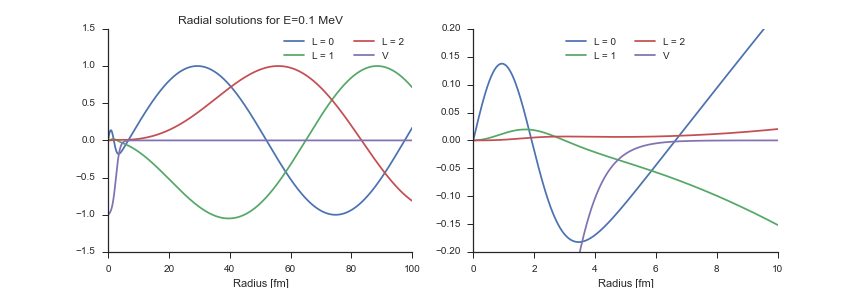
\includegraphics[width=\textwidth]{images/u_e01mev.png}
	\caption{The radial solution for $E=\SI{0.1}{MeV}$. The potential (normalized to 1) has been plotted in purple to show where the influence of the interaction dies out. The right-hand graph shows the behavior near the origin.}
	\label{fig:u01}
\end{figure}

\begin{figure}
	\centering
	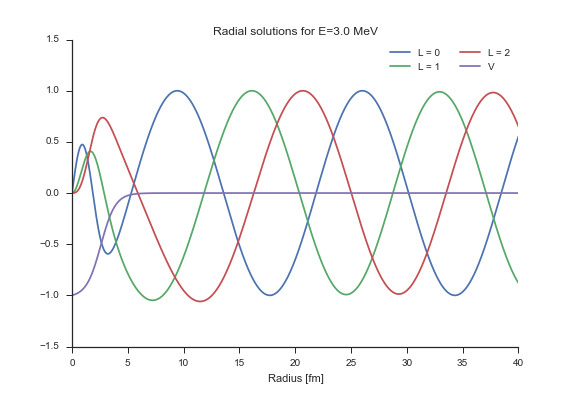
\includegraphics[width=0.8\textwidth]{images/u_e3mev.png}
	\caption{The radial solution for $E=\SI{3.0}{MeV}$. The potential (normalized to 1) has been plotted in purple to show where the influence of the interaction dies out.}
	\label{fig:u3}
\end{figure}

At large radial coordinates, the solutions become sinusoidal, as expected. Near the origin, we see that the distance to the first node increases for increasing angular momentum. This is caused by the centrifugal barrier.


\section*{Part 4}

Figure \ref{fig:phase} below shows the energy dependence of the phase shifts for $l=0,1,2$ between \SI{0.1}{MeV} and \SI{4.0}{MeV}. 

\begin{figure}
	\centering
	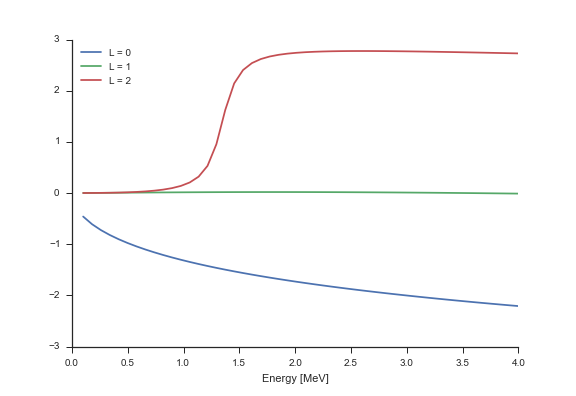
\includegraphics[width=0.8\textwidth]{images/phaseshifts.png}
	\caption{The phase shifts as a function of energy. The shape of the curve for $L=2$ suggests a resonance around 1.4 MeV.}
	\label{fig:phase}
\end{figure}

The phase shifts for $l=0$ simply reflect the fact that scattering is more likely at lower energies when angular momentum is not a factor. 

For $l=1$, we see essentially zero phase shift for all energies. This suggests that there is no interaction for this value of angular momentum.

For $l=2$, we see one resonance around \SI{1.4}{MeV}. This is indicated by the rapid change in phase and the arctangent-like shape of the curve.

\section*{Part 5}

The phase shift $\delta_l(E)$ follows the expected Breit-Wigner form for a resonance at $E$ around \SI{1.4}{MeV} with a width of around \SI{250}{keV}.  If we were to use this phase shift to calculate the scattering cross section as a function of energy, we would see a peak at this energy.  Experimental results (from \url{nndc.bnl.gov}) show a $5/2^+$ resonance at \SI{1.783}{MeV} with a width of \SI{100}{keV}, which could correspond to the $l=2$ resonance we see in our simplified theoretical model.

\end{document}